\documentclass[11pt]{article}
\usepackage[T1]{fontenc}
\usepackage{lmodern,microtype}
\usepackage[margin=1in]{geometry}
\usepackage{amsmath,amssymb,amsthm,mathtools}
\usepackage{booktabs,array,enumitem,longtable}
\usepackage{tikz,xcolor,url}
\usetikzlibrary{arrows.meta,positioning,calc,shapes.geometric}
\usepackage[colorlinks=true,linkcolor=blue!55!black,
  citecolor=green!35!black,urlcolor=blue!55!black]{hyperref}
\usepackage[nameinlink,noabbrev]{cleveref}

\setlist{nosep}
\setlength{\parskip}{0.35em}
\setlength{\parindent}{0pt}
\setlength{\emergencystretch}{3em}
\newcolumntype{L}[1]{>{\raggedright\arraybackslash}p{#1}}

\newtheorem{theorem}{Theorem}[section]
\newtheorem{proposition}[theorem]{Proposition}
\newtheorem{lemma}[theorem]{Lemma}
\newtheorem{corollary}[theorem]{Corollary}
\newtheorem{definition}[theorem]{Definition}
\theoremstyle{remark}
\newtheorem{remark}[theorem]{Remark}

\newcommand{\G}{\mathbb Z_2\times\mathbb Z_2}
\newcommand{\X}{\mathcal X}
\newcommand{\R}{\mathbb R}
\newcommand{\C}{\mathbb C}
\newcommand{\M}{\mathcal M}
\newcommand{\V}{\mathcal V}
\newcommand{\Dplus}{\mathcal D_+}
\newcommand{\Dct}{\mathcal D_{\mathrm{CT}}}
\newcommand{\PhiN}{\Phi_N}
\newcommand{\preceqplus}{\preceq_+}
\newcommand{\bowtieplus}{\mathbin{\bowtie}_+}
\newcommand{\preceqct}{\preceq_{\mathrm{CT}}}
\newcommand{\bowtiect}{\mathbin{\bowtie}_{\mathrm{CT}}}
\newcommand{\trianglerel}{\equiv_\triangle}
\newcommand{\1}{\mathbf 1}
\newcommand{\xor}{\mathbin\oplus}

\definecolor{retic}{RGB}{176,43,43}
\definecolor{treecol}{RGB}{37,85,155}
\tikzset{
  vertex/.style={circle,draw,minimum size=5.5mm,inner sep=1pt,fill=white},
  treev/.style={vertex,draw=treecol,thick},
  reticv/.style={vertex,draw=retic,thick,double},
  leaf/.style={circle,draw,minimum size=4.8mm,inner sep=.4pt,fill=white},
  ordinary/.style={line width=.7pt},
  reticedge/.style={-{Stealth[length=2mm]},draw=retic,line width=.85pt}
}

\hypersetup{
  pdftitle={Generic Identifiability and Directed Containment for Strongly
    Tree-Child Level-2 Networks under the Kimura Two-Parameter Model:
    The Principal Positive Domain and Strict Continuous Time},
  pdfauthor={Alec Kriebel},
  pdfsubject={Generic identifiability of level-2 phylogenetic networks under K2P},
  pdfkeywords={phylogenetic networks, Kimura two-parameter model,
    identifiability, level-2 networks, strongly tree-child networks,
    semi-directed networks, computer-assisted proof}
}

\title{Generic Identifiability and Directed Containment for\\
Strongly Tree-Child Level-2 Networks under the\\
Kimura Two-Parameter Model\\
\large The Principal Positive Domain and Strict Continuous Time}
\author{Alec Kriebel\\
\small Independent Researcher\\
\small ORCID: \href{https://orcid.org/0009-0001-9320-500X}
{0009-0001-9320-500X}\\
\small Corresponding email: \href{mailto:me@aleckriebel.com}
{me@aleckriebel.com}}
\date{August 2026}

\begin{document}
\maketitle

\begin{abstract}
We classify regular full-dimensional stochastic containment among binary
standard semi-directed strongly tree-child level-2 phylogenetic networks
under the Kimura two-parameter (K2P) model.  On the principal positive
Fourier domain
\[
 \Dplus=\{(s,g):0<s<1,\ 0<g<1,\ g>2s-1\},
\]
a directed containment germ exists if and only if the two labelled networks
are isomorphic after independently redirecting ordinary three-cycle factors.
The same condition is equivalent to a common full-dimensional regular germ;
in particular, no proper one-sided containment occurs.  It follows that the
semi-directed topology is generically identifiable modulo ordinary triangle
redirection, and that its structural triangle class is exactly reconstructible
away from a proper algebraic exceptional set.

The proof combines pointwise displayed-quartet inequalities and exact
whole-map \(\mathcal T_i\) identities, an exact two-sector bridge-fibre
theorem, physical marginal submersions, a finite
localization argument, and a bounded graph-to-algebra classification of cycle
and theta factors.  The bounded classification is computer-assisted: every
directed primitive relation, rank exclusion, restoration parent, transport,
and one-/two-port probe is represented by an exact certificate and has a
separately implemented replay and targeted mutation tests.  We state this
residue explicitly rather than replacing it by an unproved hand-orbit claim.
The classification transfers to the strict continuous-time domain
\(0<s<1,\ s^2<g<1\).  Finally, for every \(n\ge3\) we give two weakly but not
strongly tree-child level-2 networks whose continuous-time K2P images share a
regular germ of dimension \(4n-3\), proving that strong tree-childness is a
sharp hypothesis.
\end{abstract}

\noindent\textbf{Keywords.} phylogenetic networks; Kimura two-parameter
model; generic identifiability; directed containment; level-2 networks;
strongly tree-child networks; algebraic statistics; computer-assisted proof.

\medskip
\noindent\textbf{MSC 2020.} 92B10, 62R01, 14P10, 05C05.

\section{Introduction}\label{sec:introduction}

Phylogenetic networks model reticulate evolutionary events such as
hybridization, recombination, and lateral transfer.  A network-based Markov
model assigns a site-pattern distribution to each choice of topology, edge
parameters, and inheritance probabilities.  The basic information question
is whether different topologies can generate the same distributions, or more
strongly, whether one open model image can contain a full-dimensional regular
piece of another.

The Kimura two-parameter model was introduced to distinguish transition and
transversion rates while retaining a uniform stationary distribution
\cite{Kimura1980}.  Its group-based Fourier form follows the general
framework of Evans and Speed and of Sturmfels and Sullivant
\cite{EvansSpeed1993,SturmfelsSullivant2005}.  Algebraic invariants and
Jacobian or algebraic-matroid methods have separated important network
classes, including single-cycle and level-1 networks
\cite{GrossLong2018,HolleringSullivant2021,GrossEtAl2021}.  Recent work proves
full K2P identifiability for level-1 networks modulo triangle redirection
\cite[Theorem~4.9]{BritsEtAl2026}.  Three-sunlet group-based varieties have also been
studied directly \cite{CoxGrossMartin2025}.
At level two, invariant calculations for simple and semisimple networks and
quartet-based reconstruction for outer-labelled planar galled networks give
complementary partial classifications
\cite{Ardiyansyah2021,HoltgrefeEtAl2025Quartets}.

Huber et al.~\cite[Lemma~4.2 and Figure~8]{HuberEtAl2025} classify the two
semi-directed level-2 generator types underlying simple strict level-2
networks.  Englander et al.~\cite{EnglanderEtAl2026} use these generators in
their strongly tree-child analysis.  Their Propositions~2.9--2.10 and
Theorem~2.11 prove, for JC and K2P, pointwise separation of networks with
different displayed-quartet sets; their Corollary~2.12 combines this
separation with the quarnet structure to recover the labelled tree of blobs.
Their main level-2 algebraic classification is for JC.

The directed ported refinement used here, and also in the companion JC
classification~\cite{KriebelJC2026}, additionally records the incoming
source, internal reticulation events, path-sink child roles, minimum strong
repairs, and ordered boundary words.  This refinement produces the four event
placements \(\theta_0,\ldots,\theta_3\).  The present work proves that graph
layer in \cref{prop:cores} and rebuilds every algebraic layer for K2P, whose
nonzero Fourier characters split into two orbits rather than one.

Our classification concerns a source-relative analytic containment with a
physical target section, not merely inclusion of complex varieties.  This
distinction is important.  Boundary degenerations, lower-dimensional
intersections, and equality of Zariski closures do not by themselves create
an open stochastic containment.  Conversely, an open containment cannot be
excluded only by comparing generic dimensions when the source can enter an
exceptional target locus.  The pointwise topology inequalities and the
physical localization theorem below address these issues directly.

The proof has five layers.
\begin{enumerate}[label=\textbf{L\arabic*.}]
  \item Exact quartet and three-leaf inequalities recover the labelled
        decorated tree of blobs at every strict physical point.
  \item Positive rank-one bridge factorizations yield precisely two
        incidence scales per component--bridge incidence: one for the
        \(\{C,T\}\) sector and one for the \(G\) sector.  Explicit analytic
        normalizers and strict serial subdivisions turn the ambient quotient
        into a physical local product chart.
  \item Marginal maps are physical submersions.  A finite semialgebraic-cover
        argument localizes a global directed relation to one incoming and
        completion type of each primitive factor; remote components cannot
        cancel a local certificate.
  \item A bounded exact computation classifies every primitive four- and
        five-port direction and discharges every fixed-full restoration
        obligation.  Separately certified one- and two-port probes recover
        arbitrary labelled subdivision words.
  \item Ordinary triangle orientations share a strict rank-nine K2P germ.
        Contextual contraction and simultaneous physical bridge gluing give
        the converse global relation.
\end{enumerate}

The computer-assisted fourth layer is finite and exact, but it remains a
load-bearing residue.  Its theorem object records both graphs, direction,
incoming roles, port permutations, omitted roles, transports, polynomial or
rank certificates, and parent--child provenance.  The reader supplement gives
the census, proof schema, representative examples, replay commands, and a
claim-to-artifact crosswalk.  No claim that the millions of raw presentations
have already been reduced to a complete short hand proof is made here.

\section{Networks, K2P, and observational relations}\label{sec:definitions}

\subsection{Rooted and semi-directed conventions}

\begin{definition}[Rooted binary network]\label{def:rooted}
Let \(\X\) be a finite set of leaf labels.  A rooted binary phylogenetic
network on \(\X\) is a finite directed acyclic graph without parallel arcs in
which the root has bidegree \((0,2)\), each tree vertex has bidegree \((1,2)\),
each reticulation has bidegree \((2,1)\), and each leaf has bidegree \((1,0)\)
and a unique label in \(\X\).  Every vertex is reachable from the root.  We
require the root to be the lowest stable ancestor of the labelled leaves:
it lies on every root-to-leaf path, and no proper descendant has that
property.
The presentation is \emph{tree-child} if every internal vertex has a tree
vertex or leaf as a child.
\end{definition}

\begin{definition}[Standard semi-directed network]\label{def:semidirected}
From a rooted binary network, mark every arc entering a reticulation, undirect
every other arc, delete the binary root, and merge its two incident arcs into
one edge.  At either endpoint retain exactly the arrowhead present before root
deletion.  A presentation is admissible here only when this one suppression
produces a simple binary mixed graph: it creates neither a loop nor a parallel
edge and loses no reticulation arrowhead.  No later exhaustive cleanup is part
of this operation.  The resulting labelled mixed graph is a \emph{standard
semi-directed network}.  An \emph{admissible rooting} of it is a rooted binary
network whose one-step suppression is exactly that mixed graph.
\end{definition}

Isomorphisms preserve leaf labels, ordinary edges, retained arrowheads, and
vertex roles.  This fixed-mixed-graph convention is the one used by the
primitive compiler.  Restriction to a leaf subset is a different operation:
after choosing displayed reticulation parents, one may prune unlabelled dead
ends and suppress unlabelled bivalent vertices.  Such cleanup does not enlarge
the admissible-rooting set of the original mixed graph.  Standard references
on rooted and semi-directed conventions include
\cite{SempleSteel2003,HoltgrefeEtAl2026}.

\begin{definition}[Weak and strong tree-childness]\label{def:strong}
A standard semi-directed network is \emph{weakly tree-child} when at least one
admissible rooting is tree-child.  It is \emph{strongly tree-child} when it has
an admissible rooting and every admissible rooting is tree-child.
\end{definition}

\begin{lemma}[No-omnian criterion]\label{lem:no-omnian}
In the binary fixed convention, a standard semi-directed network with an
admissible rooting is strongly tree-child if and only if every tail of a
retained reticulation edge is incident with two ordinary edges.
\end{lemma}

\begin{proof}
If a tail fails the condition, binary degree leaves two cases.  It is a
reticulation with a reticulation child, in which case every admissible rooting
already fails tree-childness; or it is an ordinary vertex tailing two retained
edges.  A rooting away from those two edges makes both reticulations children
of that vertex.  If an admissible rooting instead subdivides one retained
edge, move the root to the tail's unique ordinary incidence.  The old root
suppresses back to the first retained edge, all other arrowheads are fixed,
and acyclicity is preserved because the tail had indegree one.  The resulting
admissible rooting has two reticulation children at the tail and is not
tree-child.  Thus failure of the incidence condition prevents strong
tree-childness.

Conversely, assume the condition.  In any admissible rooting, an ordinary
vertex with one reticulation child has, besides that retained edge, two
ordinary incidences; one is its parent and the other is a tree or leaf child.
A reticulation cannot tail a retained edge, since its two incoming retained
edges plus such an outgoing retained edge would leave no two ordinary
incidences.  Hence it has an ordinary child.  A root inserted on an ordinary
edge has a tree or leaf endpoint, while a root inserted on an edge entering a
reticulation has the ordinary tail as a tree child.  A root with two
reticulation children would suppress to an edge with two arrowheads, excluded
by \cref{def:semidirected}.  Every admissible rooting is therefore tree-child.
\end{proof}

This is the local criterion used in the primitive repair table of
\cref{sec:finite}.

A \emph{bridge} is an edge whose deletion disconnects the underlying graph.
A \emph{blob} is a maximal nontrivial biconnected block.  A network is
\emph{level two} when every blob contains at most two reticulations.  Contract
each blob and retain the intervening ordinary branching components; the
resulting labelled tree is the \emph{tree of blobs}.  Cutting a blob from the
network turns every incident bridge into a labelled boundary \emph{port}.  A
\emph{complete ported factor} retains every physical port, including a child
port below each path-sink reticulation.

\begin{definition}[Ordinary triangle relation]\label{def:triangle}
An ordinary triangle redirection changes only which vertex of a three-cycle
factor incident with exactly three external arms is reticulate and redirects
the two arrowheads entering it.  Write \(N\trianglerel N'\) when the labelled
decorated trees of blobs agree, corresponding nontriangle factors are
labelled mixed-graph isomorphic, and each remaining corresponding factor
differs by such a redirection, with coherent boundary transports.
\end{definition}

This is a structural quotient.  It does not assert equality of the complete
stochastic images of two redirected networks.

\subsection{The K2P network map}

Identify the four states and their characters with
\(\G=\{0,C,G,T\}\), where addition is the Klein-four-group operation.  A K2P
edge \(e\) has Fourier spectrum
\[
 \widehat f_e=(1,s_e,g_e,s_e).
\]
Equivalently, if \(M_e(x,y)=f_e(y-x)\), inverse Fourier transformation gives
\begin{equation}\label{eq:inverse-fourier}
 f_e(0)=\frac{1+2s_e+g_e}{4},\quad
 f_e(C)=f_e(T)=\frac{1-g_e}{4},\quad
 f_e(G)=\frac{1-2s_e+g_e}{4}.
\end{equation}
The root state is uniform.  At each reticulation \(r\), one incoming edge is
selected with probability \(\lambda_r\in(0,1)\) and the other with probability
\(1-\lambda_r\).  A vector of choices \(\sigma\) gives a displayed tree
\(T_\sigma\), with positive weight \(w_\sigma\).

For a character assignment \(\mathbf h=(h_i)_{i\in\X}\), the Fourier
network parameterization is
\begin{equation}\label{eq:k2p-fourier}
 q_N(\mathbf h)=
 \begin{cases}
 \displaystyle
 \sum_\sigma w_\sigma
 \prod_{e\in T_\sigma}
 \widehat f_e\!\left(\xor_{i\in A_e}h_i\right),
 &\xor_{i\in\X}h_i=0,\\[2mm]
 0,&\text{otherwise},
 \end{cases}
\end{equation}
where \(A_e\mid A_e^c\) is the displayed-tree split.  This is a polynomial
map in the Fourier edge coordinates and inheritance probabilities.

Strict positivity of all four entries in \eqref{eq:inverse-fourier} is
equivalent to
\[
 1-g>0,\qquad 1+2s+g>0,\qquad 1-2s+g>0.
\]
The principal positive-eigenvalue component is
\begin{equation}\label{eq:Dplus}
 \Dplus=\{(s,g):0<s<1,\ 0<g<1,\ g>2s-1\}.
\end{equation}
Every edge in the main theorem lies in \(\Dplus\), and every inheritance
probability lies in \((0,1)\).  Write \(\Theta_+(N)\) for this open parameter
space, \(\Phi_N\) for \eqref{eq:k2p-fourier}, and
\(\M_+(N)=\Phi_N(\Theta_+(N))\).  Put
\[
 d_N=\max_{\theta\in\Theta_+(N)}\operatorname{rank}D\Phi_N(\theta).
\]
A source parameter is \emph{regular} if its Jacobian rank is \(d_N\).

\subsection{Directed containment and common germs}

\begin{definition}[Regular analytic relations]\label{def:relations}
Write \(N\preceqplus N'\) if there are a regular source point
\(\theta_0\in\Theta_+(N)\), a connected open neighborhood
\(U\subseteq\Theta_+(N)\) on which \(\Phi_N\) has rank \(d_N\), and a real
analytic physical target section \(\sigma:U\to\Theta_+(N')\) satisfying
\[
 \Phi_N=\Phi_{N'}\circ\sigma\qquad\text{on }U.
\]
Write \(N\bowtieplus N'\) if the two images contain a common analytic germ
which is regular and full-dimensional in both images and which has physical
analytic sections from both parameter spaces.
\end{definition}

These relations are deliberately stronger than nonempty image intersection.
They are distinct from equality of complete stochastic images, inclusion or
equality of complex Zariski closures, lower-dimensional coincidence, and
boundary-only intersection.  The main theorem proves that \(\preceqplus\) is
symmetric inside the stated class; symmetry is not built into the definition.

\section{Physical domain and pointwise topology recovery}\label{sec:pointwise}

\begin{lemma}[Strict subdivision]\label{lem:subdivision}
Every \((s,g)\in\Dplus\) factors into two strict pairs in \(\Dplus\).  More
precisely, for all sufficiently small \(\varepsilon>0\),
\[
 (s_B,g_B)=(1-\varepsilon,1-\varepsilon),\qquad
 (s_A,g_A)=\left(\frac{s}{1-\varepsilon},
                  \frac{g}{1-\varepsilon}\right)
\]
are in \(\Dplus\) and multiply coordinatewise to \((s,g)\).
\end{lemma}

\begin{proof}
At \(\varepsilon=0\), the second pair is the given interior point and the
first approaches the identity from within \(\Dplus\).  All defining
inequalities are strict and continuous.  Hence they persist on a sufficiently
small positive interval.  This avoids the false general assertion that
coordinatewise square roots of every strict stochastic K2P edge are physical.
\end{proof}

\begin{lemma}[Root movement]\label{lem:root-movement}
For symmetric K2P, the map \(\Phi_N\) is unchanged by moving the root to any
admissible rooting of the same standard semi-directed graph.
\end{lemma}

\begin{proof}
Reverse only ordinary arcs on an old-to-new root path.  K2P transition
matrices are symmetric and the root distribution is uniform, so every
displayed-tree probability is unchanged.  Use \cref{lem:subdivision} at the
new root and suppress the old root.  If the old root is adjacent to an edge
entering a reticulation, inspect each switching.  When that parent is chosen,
the two old root arms enter only through their serial products.  When the
other parent is chosen, the remaining one-child stem subtends every observed
leaf, carries total Fourier character zero, and contributes multiplier one.
Thus every summand in \eqref{eq:k2p-fourier} is unchanged.  Strong
tree-childness supplies the admissible tree-child rootings used later, but
the algebraic invariance is reversibility, subdivision, and switching.
\end{proof}

\subsection{Whole-map quartet separation}

Let the three quartet splits be
\(A=12\mid34\), \(B=13\mid24\), and \(C=14\mid23\).  Define
\begin{align}
 F_A&=q_{CCCC}-q_{CCTT},\label{eq:quartet-F}\\
 G_B&=q_{CCCC}-q_{CCTT}-q_{CTTC}+q_{CTCT}.
 \label{eq:quartet-G}
\end{align}

\begin{lemma}[Displayed-quartet sign theorem]\label{lem:quartet}
On a strict physical K2P quartet tree, \(F_A\) is zero on topology \(A\)
and strictly positive on \(B\) and \(C\).  The polynomial \(G_B\) is zero
on \(A\) and \(C\) and strictly positive on \(B\).  Consequently two strict
network restrictions with different displayed-quartet sets have disjoint
physical images.
\end{lemma}

\begin{proof}
The equal K2P character sector in the convention of
\eqref{eq:inverse-fourier} is \(\{C,T\}\).  Let
\(P=s_1s_2s_3s_4>0\), and let \(g_I\in(0,1)\) be the singleton-sector
eigenvalue on the internal quartet edge.  Direct substitution in
\eqref{eq:k2p-fourier} gives the complete pullback table
\[
\begin{array}{c|ccc}
 &A&B&C\\ \hline
F_A&0&P(1-g_I)&P(1-g_I)\\
G_B&0&2P(1-g_I)&0.
\end{array}
\]
Thus the asserted zeros and strict signs hold on all of \(\Dplus\).  Leaf
permutations give \(F_t,G_t\) for every split \(t\); the global
\(C\leftrightarrow T\) symmetry gives the equivalent character transport.
These are the current-paper coordinates corresponding to the equal-sector
formulas in Englander et al.

A network tensor is a positive mixture of all displayed-tree tensors.  If one
displayed set is the singleton \(\{t\}\) and the other contains a different
topology, \(F_t\) is zero on the first map and positive on the second.  If
both displayed sets have size at least two and differ, choose a topology
\(t\) present in one and absent from the other; the corresponding \(G_t\)
is positive on the first mixture and zero on the second.  These cases exhaust
the nonempty subsets of the three quartet topologies.  This is the explicit
K2P specialization of the pointwise theorem of
Englander et al.~\cite[Propositions~2.9--2.10 and
Theorem~2.11]{EnglanderEtAl2026}.
\end{proof}

Marginalization sets omitted Fourier characters to zero.  Equality of full
tensors would therefore imply equality of every quartet marginal.  By
\cite[Corollary~2.12]{EnglanderEtAl2026}, \cref{lem:quartet} gives:

\begin{corollary}[Tree-of-blobs recovery]\label{cor:tree-blobs}
Every tensor in the strict image determines the labelled tree of blobs
pointwise.  In particular, \(N\preceqplus N'\) forces the same labelled tree
of blobs.
\end{corollary}

\subsection{The whole-map \texorpdfstring{\(\mathcal T_i\)}{Ti} polynomial}

For a three-leaf tensor use character zero \(0\) and put
\[
 X_h=q_{hh0},\qquad Y_h=q_{h0h},\qquad Z_h=q_{0hh}\quad(h=s,g),
 \qquad V=q_{CTG},
\]
where \(h=s\) means either member of the equal \(\{C,T\}\) sector and
\(h=g\) means \(G\).  Define
\begin{equation}\label{eq:Ti}
 \mathcal T_3=V^2X_g-X_s^2Y_gZ_g.
\end{equation}

\begin{lemma}[Whole-map tree--sunlet strict sign]\label{lem:Ti}
The polynomial \(\mathcal T_3\) vanishes on every three-leaf K2P tree.  For
the three-sunlet whose reticulation is incident with leaf three, write its
Fourier map as
\begin{equation}\label{eq:sunlet-map}
 q_{xyz}=a_xb_yc_z\{\delta f_y d_z+(1-\delta)f_xe_z\},
 \qquad x+y+z=0,
\end{equation}
with edge spectra \(a,b,c,d,e,f\) and \(0<\delta<1\).  Then
\begin{equation}\label{eq:Ti-factor}
 \mathcal T_3=
 -a_s^2b_s^2a_gb_gc_g^2f_s^2
 \delta(1-\delta)d_ge_g(1-f_g)^2<0.
\end{equation}
The other two orientations have the corresponding leaf-permuted
certificates.
\end{lemma}

This lemma is an identity on the original full Fourier maps.  It is not a
classifier obtained by rooting and pruning a three-leaf mixed-graph
restriction; that historically tempting shortcut is false for some restored
and probe presentations.

\begin{proof}
For a three-leaf tree with pendant spectra \(a,b,c\),
\[
 X_s=a_sb_s,\quad X_g=a_gb_g,\quad
 Y_g=a_gc_g,\quad Z_g=b_gc_g,\quad V=a_sb_sc_g,
\]
so the two monomials in \eqref{eq:Ti} agree.  For the sunlet, substitute
\eqref{eq:sunlet-map} into \eqref{eq:Ti}.  After removing the common positive
monomial, the remaining identity is
\[
 f_g\{\delta d_g+(1-\delta)e_g\}^2
 -\{\delta d_g+(1-\delta)f_ge_g\}
  \{\delta f_gd_g+(1-\delta)e_g\}
 =-\delta(1-\delta)d_ge_g(1-f_g)^2.
\]
This gives \eqref{eq:Ti-factor}.  Every factor after the leading minus sign
is strictly positive on \(\Dplus\).
\end{proof}

Thus the ordinary-vertex/three-sunlet decoration of each degree-three node is
pointwise determined.  A strongly tree-child theta factor has at least four
physical boundaries, so it cannot be confused with an ordinary three-boundary
factor.  Together with \cref{cor:tree-blobs}, this recovers the complete
labelled decorated tree of blobs before any finite algebraic classification.

\section{The complete two-sector bridge fibre}\label{sec:bridges}

Cut every bridge of the common decorated tree of blobs.  Its
component-incidence graph is a tree \(T\).  For a component \(v\), let
\(P_v\) be its normalized Fourier boundary tensor, including retained physical
blocks and one character \(h_e\) for each incident bridge; thus \(P_v(0)=1\).
For a bridge \(e=uv\), put
\[
 k_e(h)=
 \begin{cases}
 1,&h=0,\\
 s_e,&h\in\{C,T\},\\
 g_e,&h=G.
 \end{cases}
\]
Character conservation makes the global contraction
\begin{equation}\label{eq:bridge-contraction}
 Q(\mathbf h)=
 \prod_{v\in V(T)}P_v(\mathbf h|_v)
 \prod_{e\in E(T)}k_e(h_e),
\end{equation}
where \(h_e\) is the group sum of the leaf characters on either side of the
bridge cut.

Call a component \emph{marked} when its local tensor retains at least one
physical boundary block that can carry a compensating sector character in an
anchor entry; otherwise call it \emph{unmarked}.  Unmarked retained components
have bridge degree at least three.

\begin{lemma}[Paired-sector uniqueness]\label{lem:paired-scale}
Let a positive normalized component tensor and its incidence-scaled image
both be invariant under \(C\leftrightarrow T\).  If the scale at incidence
\(e\) is \(c_e(h)\), then \(c_e(C)=c_e(T)\) for every retained component.
\end{lemma}

\begin{proof}
Normalize \(c_e(0)=1\) and write
\(\rho_e=c_e(C)/c_e(T)>0\).  If the component has a retained physical block,
compare conservation-supported positive entries carrying \(C,C\), and then
\(T,T\), at that block and incidence \(e\), with zero elsewhere.  Invariance
before and after scaling gives \(\rho_e=1\).

For an unmarked degree-\(d\) component, compare the analogous entries at
each pair \(e\ne f\).  This gives \(\rho_e\rho_f=1\).  Three distinct
incidences and positivity imply every \(\rho_e=1\).  The only residual at
degree two would be \((\rho_1,\rho_2)=(t,t^{-1})\).  No such unmarked factor
is retained: cycle, theta, and ordinary components have at least three
physical incidences in the strong class, while the only simple two-boundary
theta \(K_4-e\) has no tree-child rooting.
\end{proof}

\begin{theorem}[Complete positive bridge fibre]\label{thm:bridge-fibre}
On the positive normalized K2P component-tensor locus, the complete fibre of
\eqref{eq:bridge-contraction} is exactly
\begin{align}
 P_v&\longmapsto P_v
 \prod_{e\ni v}
 a_{v,e}^{\1[h_e\in\{C,T\}]}
 b_{v,e}^{\1[h_e=G]},\label{eq:bridge-action-P}\\
 s_e&\longmapsto\frac{s_e}{a_{u,e}a_{v,e}},
 &g_e&\longmapsto\frac{g_e}{b_{u,e}b_{v,e}},
 \label{eq:bridge-action-edge}
\end{align}
with positive incidence scales \(a_{v,e},b_{v,e}\).  There is no additional
positive continuous or discrete gauge, the action is free on every retained
component, and the bridge tree has no two-sector holonomy.  On physical
networks, the fibre is the intersection of this orbit with all local,
inheritance, arm, bridge, and K2P inequalities.
\end{theorem}

\begin{proof}
Cut one bridge and fix its character.  The corresponding flattening block is
a positive rank-one matrix.  Positive rank-one factorization is unique up to
one positive scalar.  All-zero normalization fixes the zero-character scalar;
\cref{lem:paired-scale} identifies the \(C\) and \(T\) scalars, while the
\(G\) scalar remains independent.  Root \(T\) temporarily and peel its leaf
components.  In the paired and singleton sectors separately, the resulting
cut scalars assign one positive scale to every component incidence and give
exactly \eqref{eq:bridge-action-P}--\eqref{eq:bridge-action-edge}.  Induction
reaches every component, so no vertex-coupled scale or holonomy remains.
Direct cancellation proves the converse, and the observable sector labels
exclude a discrete interchange.

It remains to prove freeness and analytic normalization.  A marked component
uses, for each incidence, a positive conservation-supported entry carrying
the chosen sector character at that incidence and at one retained physical
block; its exponent matrix is the identity.  For an unmarked component of
degree \(d\ge3\), use in either sector the pair anchors
\[
 (1,2),(1,3),(2,3),(1,4),\ldots,(1,d).
\]
Their exponent matrix has leading determinant \(-2\) and rank \(d\).  If the
observed anchor ratios are \(r_{ij}\), the unique positive scales are
\begin{equation}\label{eq:bridge-normalizer}
 a_1=\sqrt{\frac{r_{12}r_{13}}{r_{23}}},\quad
 a_2=\sqrt{\frac{r_{12}r_{23}}{r_{13}}},\quad
 a_3=\sqrt{\frac{r_{13}r_{23}}{r_{12}}},\quad
 a_k=\frac{r_{1k}}{a_1}.
\end{equation}
Apply the same formula independently in the singleton sector.  Positivity
makes the normalizers real analytic.  The excluded degree-two stabilizer is
the only possible failure of freeness.
\end{proof}

The normalizers first produce an ambient positive-tensor quotient.  The next
lemma supplies the physically essential saturation.

\begin{lemma}[Physical local product chart]\label{lem:physical-product}
Near every regular physical point, the quotient in
\cref{thm:bridge-fibre} is a physical local product chart.
\end{lemma}

\begin{proof}
Split every effective bridge pair \((s,g)\) into three serial pairs
\[
 (\alpha_u,\beta_u),\qquad
 \left(\frac{s}{\alpha_u\alpha_v},
       \frac{g}{\beta_u\beta_v}\right),\qquad
 (\alpha_v,\beta_v).
\]
Choose both endpoint pairs sufficiently near \((1,1)\) that all three lie
strictly in \(\Dplus\), using \cref{lem:subdivision} twice.  Strictness is
open; hence the four endpoint coordinates vary independently in a
neighborhood while the residual pair remains physical.  Absorbing the
endpoint factors into the adjacent tensors realizes all four incidence-scale
directions.  Perform this independently on the bridge tree and intersect the
ambient quotient with a constant-rank physical parameter chart.
\end{proof}

For later use we now make the localized relation precise.  If \(H\) is a
complete ported factor, let \(\Theta_+(H)\) contain its internal and retained
arm K2P pairs and its inheritance parameters, and let
\(P_H(\theta)\), with \(P_H(0)=1\), be its normalized boundary Fourier
tensor.  The positive incidence torus
\(A_H=(\mathbb R_{>0}^2)^{\operatorname{ports}(H)}\) acts by
\[
 P_H(\mathbf h)\longmapsto P_H(\mathbf h)
 \prod_e a_e^{\1[h_e\in\{C,T\}]}
          b_e^{\1[h_e=G]}.
\]
On any positive anchor chart, \eqref{eq:bridge-normalizer} gives an analytic
slice for this action.  Write \(\overline\Phi_H\) for the resulting slice map
and
\[
 d_H=\max_{\theta\in\Theta_+(H)}
       \operatorname{rank}D\overline\Phi_H(\theta).
\]
After fixing a physical port bijection, define \(H\preceqplus H'\) exactly as
in \cref{def:relations}, with \(\Phi_N,\Phi_{N'}\) replaced by
\(\overline\Phi_H,\overline\Phi_{H'}\), a source neighborhood of rank
\(d_H\), and a physical analytic target section.  This definition is
independent of the anchor chart: two such slices differ only by the free
analytic incidence action of \cref{thm:bridge-fibre}.  The notation
\(H\trianglerel H'\) means the restriction of \cref{def:triangle} to the two
complete ported factors with that same port bijection.  Thus every local
relation used below is a relation between quotient model germs, not merely a
comparison of abstract graphs.

\section{Marginals, localization, and no compensation}\label{sec:localization}

\begin{lemma}[Paired marginal submersion]\label{lem:marginal}
For every \(m\ge1\), the serial-edge map
\[
 ((s_1,g_1),\ldots,(s_m,g_m))
 \longmapsto\left(\prod_i s_i,\prod_i g_i\right)
\]
maps \(\Dplus^m\) onto \(\Dplus\), has differential rank two, and has a
local physical analytic section.
\end{lemma}

\begin{proof}
First the product of physical factors remains physical.  It is enough to
check two factors.  Put \(S=s_1s_2\) and \(G=g_1g_2\).  Positivity and the
upper bounds are immediate.  If \(S\leq1/2\), then \(G>2S-1\) is automatic.
If \(S>1/2\), then both \(s_i>1/2\), and
\[
 G>(2s_1-1)(2s_2-1)
  =(2S-1)+2(1-s_1)(1-s_2)>2S-1.
\]
Induction proves that the displayed product map lands in \(\Dplus\).

The case \(m=1\) is immediate.  Given \((S,G)\in\Dplus\) and \(m\ge2\),
choose \(r\in(0,1)\) satisfying
\[
 \max\{S,G,2S-G,0\}<r^{m-1}<1.
\]
Use \((r,r)\) on the first \(m-1\) edges and
\((S/r^{m-1},G/r^{m-1})\) on the last.  The displayed inequalities put every
factor in \(\Dplus\), and the same fixed \(r\) works on a neighborhood of
\((S,G)\).  The \(s\)- and \(g\)-rows of the differential have disjoint
nonzero supports and are independent.
\end{proof}

\begin{proposition}[Complete graph-derived marginal descriptor]
\label{prop:marginal-descriptor}
Let \(Y\) be the retained boundary labels in any selected restriction used
below, and extend \(\mathbf x\in\G^Y\) by zero on the omitted labels.  For an
edge \(e\) and a displayed switching \(\sigma\), let
\(h_{e,\sigma}(\mathbf x)\) be the group sum below \(e\) when
\(e\in T_\sigma\), and put \(h_{e,\sigma}(\mathbf x)=\bot\) otherwise.  Define
\[
 \epsilon_e^s(\sigma,\mathbf x)
   =\1[h_{e,\sigma}(\mathbf x)\in\{C,T\}],\qquad
 \epsilon_e^g(\sigma,\mathbf x)
   =\1[h_{e,\sigma}(\mathbf x)=G].
\]
The \emph{complete visible signature} of \(e\) is the pair of these arrays
over all \((\sigma,\mathbf x)\).  Edges with the same
non-identically-zero signature form one effective product class \(E\), with
coordinates
\[
 S_E=\prod_{e\in E}s_e,\qquad G_E=\prod_{e\in E}g_e.
\]
Edges with identically zero signatures, and tensor-invisible inheritance
coordinates, are forgotten.  The exact graph transport permutes surviving
inheritance coordinates; only
when it reverses the recorded order of the two parents at a retained
reticulation does it apply \(\lambda_r\mapsto1-\lambda_r\).  Consequently the
effective restriction descriptor is a product of the paired serial maps of
\cref{lem:marginal}, coordinate projections and permutations, and these
recorded affine parent-order flips.  It maps the physical parameter domain
onto the effective child domain, is a submersion, and has local physical
analytic sections.
\end{proposition}

\begin{proof}
Here a reticulation is \emph{tensor-invisible} precisely when, after every
choice at the other reticulations is fixed, its two parent choices induce the
same retained switching and the same visible edge-sector exponent arrays for
every retained character assignment.  Only under this condition is its
inheritance coordinate forgotten; otherwise the compiler retains it.
Set omitted characters to zero in \eqref{eq:k2p-fourier} and group full
switchings by their induced switching on the retained graph.  Equal visible
signatures contribute in the same K2P sector in every monomial, hence only
through \((S_E,G_E)\).  Each invisible reticulation contributes
\(\lambda+(1-\lambda)=1\); every surviving reticulation is carried by the
exact graph transport, with a complement precisely when that transport
reverses its stored parent order.  This gives the asserted factorization.
\Cref{lem:marginal} handles each product class, coordinate projections are
submersions onto the retained coordinates, and permutations and parent flips
are analytic diffeomorphisms of the open physical domain.  The flips here are
not an inheritance-complement quotient between records: they occur only when
the certified graph transport reverses a parent order.
\end{proof}

We use the following standard semialgebraic fact in a form that makes the
finite-choice step explicit.

\begin{lemma}[Finite semialgebraic covers]\label{lem:finite-cover}
Let \(M\) be a smooth \(d\)-dimensional semialgebraic manifold and
\(S\subseteq M\) semialgebraic.  Then \(\dim S=d\) if and only if \(S\) has
nonempty relative interior.  Consequently, if a nonempty relatively open set
in \(M\) is covered by finitely many semialgebraic subsets, one member contains
a nonempty relatively open subset.
\end{lemma}

\begin{proof}
This follows from semialgebraic cell decomposition, invariance of dimension
under semialgebraic bijections, the frontier-dimension inequality, and the
fact that the dimension of a finite union is the maximum of its dimensions;
see \cite[Section~2.8]{BochnakCosteRoy1998}.
\end{proof}

\begin{proposition}[Physical localization and no compensation]
\label{prop:localization}
Suppose \(N\preceqplus N'\).  For each pair of corresponding complete ported
factors \(H,H'\), some fixed target incoming/completion type contains a
source-relative full-dimensional regular germ of the projective physical K2P
model of \(H\).  Parameters in other factors cannot compensate for a local
separator.
\end{proposition}

\begin{proof}
Choose the regular source neighborhood and physical target section from
\cref{def:relations}.  Shrink around a nonzero maximal source minor.  By
\cref{lem:physical-product}, source slice coordinates contain a product box
of local factor germs and effective bridge intervals.  Fix every coordinate
except one focal factor.  Positive bridge block factorization and the analytic
normalizers extract its projective incidence orbit intrinsically from the
global tensor.

Only finitely many target incoming roles and target completion types occur in
the primitive grammar.  Their semialgebraic realization sets cover the focal
source box, because the given target section realizes every point.  By
\cref{lem:finite-cover}, one type contains a source-open subgerm.  The
intrinsic bridge extraction does not depend on remote target coordinates, so
a polynomial or rank obstruction on the focal orbit cannot be cancelled in a
distant component.
\end{proof}

Restoration is used only under one fixed full relation.

\begin{lemma}[Fixed-full restoration]\label{lem:restoration}
Fix actual networks \(N,N'\) and a full relation \(N\preceqplus N'\).  Fix an
omitted physical label, its source insertion edge, its target attachment, and
the induced boundary transport.  Marginalizing this same relation gives one
enumerated child relation, and its source restriction is open.  Hence exact
separation of every physical child excludes the fixed full parent.
\end{lemma}

\begin{proof}
Marginalization sets the restored leaf character to zero.  The pendant factor
becomes one and all newly serial edges multiply to the old effective edge.
\Cref{prop:marginal-descriptor}, together with the identity on other source
parameters, gives a physical source-open image and retains every inheritance
coordinate that is not tensor-invisible.  The actual attachments and
transport of the fixed networks are one row of the exhaustive child
construction.
Therefore a separating certificate for every child contradicts the assumed
full relation.  This argument neither lifts an abstract selected relation nor
inverts an arbitrary target deletion map.
\end{proof}

\section{Primitive factors and the bounded exact theorem}\label{sec:finite}

\subsection{Graph reduction}

Remove the port arms of one blob and suppress ordinary bivalent vertices that
are neither local sources nor reticulation sinks.  Record every removed
port-bearing subdivision as a labelled ordered word on the resulting directed
segment.

\begin{lemma}[Root reduction to a real incoming port]\label{lem:root-reduction}
Every root-containing strongly tree-child factor has the same open projective
K2P germ as an incoming-port presentation at some real leaf-bearing boundary.
For a comparison, source and target incoming boundaries may be chosen
independently.
\end{lemma}

\begin{proof}
Starting at an admissible root, repeatedly choose a tree or leaf child.  This
reaches a labelled leaf without crossing a reticulation.  Move the root down
that ordinary path to its boundary arm.  Reversing the path creates no
directed cycle: a first re-entry would give an internal path tree vertex a
second parent.  The other old root branch reaches a leaf off the path, so no
proper descendant of the new root lies on every root-to-leaf path; the new
root is again the lowest stable ancestor.  One-step suppression returns the
same fixed mixed graph, and strong tree-childness makes the new rooting
tree-child.  \Cref{lem:root-movement} preserves the K2P map, while strict
subdivision or suppression changes only positive incidence factors on the
chosen arm.
\end{proof}

\begin{proposition}[Cycle--theta core theorem]\label{prop:cores}
Every nontrivial complete blob factor in the strong level-2 class has a cycle
core or one of four directed theta cores \(\theta_0,\theta_1,\theta_2,
\theta_3\).  It is recovered uniquely from that core, one labelled ordered
port word on each directed segment, and one child port below every path-sink
reticulation.
\end{proposition}

\begin{proof}
Move a root-containing factor to a real incoming boundary using
\cref{lem:root-reduction}.  Let \(t,r,v,e\) be its local tree vertices,
reticulations, total internal vertices, and blob edges after deleting port
arms.  Summing indegrees gives \(e=v+r-1\), and therefore
\[
 \sum_{w\in V(B)}(\deg_B(w)-2)=2e-2v=2(r-1).
\]
For \(r=1\), every blob vertex has degree two and the core is a cycle.  For
\(r=2\), exactly two vertices have degree three and every other vertex has
degree two.  Biconnectedness makes the blob three internally disjoint paths
between the two degree-three poles, hence a theta.

The incoming cut edge is ordinary.  Indeed, if an arc \(u\to R\) entering a
reticulation were a cut edge, the two root-to-parent paths together with the
other incoming arc of \(R\) would still connect \(u\) to \(R\) after deleting
\(uR\), a contradiction.  Its endpoint in the factor is therefore the unique
local tree source \(S\).  A theta pole already uses all three binary
incidences inside the blob, so \(S\) lies in the interior of one of the three
pole-to-pole paths.  An internal reticulation is necessarily a path sink:
both path sides enter it and its unique child is its boundary arm.

At most one pole is reticulate.  If both poles were reticulate, the path
containing \(S\) would point from \(S\) toward both poles, giving each pole
one incoming side.  Their remaining bidegrees would force the two event-free
paths to point in opposite directions, and those paths would form a directed
cycle.

Suppose exactly one pole \(R\) is reticulate and the other pole \(T\) is a
tree vertex.  The second reticulation is an internal sink \(X\).  If \(S\)
and \(X\) lie on different paths, their paths point respectively away from
\(S\) and toward \(X\), and the pole bidegrees force the third path from
\(T\) to \(R\); this is \(\theta_0\).  If they share a path, its only acyclic
order from \(T\) to \(R\) is
\[
 T-S-X-R.
\]
The order \(T-X-S-R\) forces the two event-free paths to have opposite
directions and hence creates a directed cycle.  Both event-free paths in the
valid case point from \(T\) to \(R\), giving \(\theta_1\).

Suppose instead that both poles are tree vertices.  The two reticulations are
internal sinks.  They cannot lie on one path: the path directions into the
two sinks would force \(S\) between them, after which the pole bidegrees force
the two event-free paths in opposite directions, again producing a directed
cycle.  Thus the sinks lie on distinct paths.  If \(S\) lies on the third
path, both poles feed both sinks, giving \(\theta_2\).  Otherwise \(S\)
shares a path with one sink; choose as first pole the pole whose other two
sides point outward.  The shared path then has order
pole--\(S\)--sink--pole and all remaining directions are forced, giving
\(\theta_3\).  Reversing the arbitrary pole names or interchanging the two
sinks yields only the displayed symmetries.  Hence no source or
reticulation-event placement is omitted.

Deleting the incoming arm and suppressing its resulting degree-two source
yields one of the two semi-directed level-2 generators classified by Huber et
al.~\cite[Lemma~4.2 and Figure~8]{HuberEtAl2025}.  The four directed
incoming-source refinements are exactly the cases above.
Reading port vertices along the oriented segments recovers the unique words.
\end{proof}

The segment templates and minimal strong repairs are:
\begin{center}
\small
\begin{tabular}{lll}
\toprule
core & directed segments in index order & minimum occupied segments\\
\midrule
cycle & \(S\!\to X,S\!\to X\) & \(\{0\},\{1\}\)\\
\(\theta_0\) & \(S\!\to U,S\!\to V,U\!\to X,V\!\to X,U\!\to V\)
 & \(\{2,3\},\{3,4\}\)\\
\(\theta_1\) & \(S\!\to U,S\!\to X,V\!\to X,U\!\to V,U\!\to V\)
 & \(\{2,3\},\{2,4\}\)\\
\(\theta_2\) & \(S\!\to U,S\!\to V,U\!\to X_0,V\!\to X_0,
 U\!\to X_1,V\!\to X_1\)
 & \(\{2,3\},\{2,5\},\{3,4\},\{4,5\}\)\\
\(\theta_3\) & \(S\!\to U,S\!\to X_0,V\!\to X_0,U\!\to X_1,
 V\!\to X_1,U\!\to V\)
 & \(\{2\},\{4\}\)\\
\bottomrule
\end{tabular}
\end{center}
Here is a direct proof that the repair table is complete.  If an occupied
segment ends at a reticulation, its last port-bearing subdivision replaces
the original core tail's reticulation incidence by an ordinary edge; the new
arrow tail has two ordinary incidences, namely its preceding segment edge and
its port arm.
Consequently an occupancy set \(A\) is valid exactly when it meets every
obstruction clause in
\[
\begin{array}{c|l}
\text{core} & \text{clauses that \(A\) must meet}\\
\hline
\text{cycle} & \{0,1\}\\
\theta_0 & \{3\},\ \{2,4\}\\
\theta_1 & \{2\},\ \{3,4\}\\
\theta_2 & \{2,4\},\ \{3,5\}\\
\theta_3 & \{2,4\}.
\end{array}
\]
For the cycle, \(S\) otherwise tails both reticulation edges and the two
unsubdivided sides are parallel.  In \(\theta_0\), segment \(3\) must be
occupied to separate the reticulation \(V\) from its reticulation child
\(X\), while \(U\) requires one of segments \(2,4\).  In \(\theta_1\),
segment \(2\) separates the reticulation stack, while one of the parallel
segments \(3,4\) must be occupied both to give \(U\) an ordinary child and
to make the mixed graph simple.  In \(\theta_2\), \(U\) requires one of
\(2,4\) and \(V\) one of \(3,5\).  In \(\theta_3\), \(V\) requires one of
\(2,4\).  All other retained-arrow tails already have two ordinary
incidences, and every path-sink child arm is retained separately.

The minimal transversals of these clause families are precisely the repair
sets displayed in the table.  Deleting any member of a displayed repair
leaves its named clause unmet, whereas every valid occupancy must meet all
the clauses.  This proves sufficiency, minimality, and exhaustiveness, up to
the displayed core symmetries, by the no-omnian criterion
\cref{lem:no-omnian}.  The reader supplement records the exact completion
grammar.

For a target core \(H\), let \(m_H\) be its number of directed segments,
\(q_H\) its path-sink count, and \(r_H\) its number of compiler
target-repair tags.  For theta targets these tags are the listed minimum
repairs; cycle targets use one untagged target convention.  If \(k\)
physical boundaries are selected and
\(\epsilon=1\) when the incoming boundary is selected
(\(\epsilon=0\) when it is marginalized), then the exact number of target
completions is
\begin{equation}\label{eq:completion-count}
 C(k,\epsilon)=\sum_H r_H\sum_{j=0}^{q_H}
 \binom{q_H}{j}
 \binom{k-\epsilon-j+m_H-1}{m_H-1}.
\end{equation}
This counts repair-tagged directed completion descriptors, not untagged mixed
graphs.  First choose the \(j\) selected path sinks and weakly distribute the
remaining \(k-\epsilon-j\) selected physical labels among the \(m_H\)
ordered segment words.  For a chosen theta repair, every required segment
whose physical word is empty then receives one deterministically named
zero-character completion leaf; an already occupied required segment
receives no extra leaf.  These completion roles consume no selected label and
therefore do not alter the stars-and-bars term.  The repair index remains part
of the raw descriptor even when two repair witnesses construct the same final
mixed graph.  Unselected path-sink roles and a marginalized incoming role
likewise receive deterministic dummy labels.  Cycle targets use the single
untagged target-repair convention; their two minimum repaired supports enter
the source multiplier rather than \(C\).

The five tuples \((m_H,q_H,r_H)\) are
\[
 (2,1,1),\ (5,1,2),\ (5,1,2),\ (6,2,4),\ (6,2,2)
\]
for the cycle and \(\theta_0,\ldots,\theta_3\), respectively.  Thus
\(C(4,1)=831\), \(C(4,0)=C(5,1)=1{,}983\), and
\(C(5,0)=4{,}155\).  Physical label permutations are applied only after
this directed-record enumeration.

\subsection{What was computed}

For clarity, a \emph{raw directed presentation} consists of the source graph,
target graph, source and target incoming modes, all selected or marginalized
physical roles, an ordered physical port permutation, the source-to-target
direction, and the boundary transport.  Canonical classes are formed only
after the raw ledger is complete.  A row may terminate only by one of the
following mutually exclusive evidence types, applied in order:
\begin{enumerate}[label=(\roman*)]
  \item a pointwise displayed-quartet or whole-map \(\mathcal T_i\) sign
        exclusion;
  \item a directed exact-rank exclusion, with a nonzero source minor and a
        symbolic target upper certificate;
  \item an exact polynomial separator, zero on the target map and nonzero at
        a strict rational source point;
  \item a fixed-full restoration obligation;
  \item a labelled mixed-graph isomorphism; or
  \item an ordinary triangle relation.
\end{enumerate}

The target completion grammar takes every primitive core, every allowed
path-sink child subset, every weak composition of the available port roles
among directed segments, every theta minimum-repair tag (and the single
untagged cycle convention), and either a selected incoming boundary or a
marginalized incoming role.  It produces 831
selected-incoming and 1,983 marginalized-incoming four-port targets.  At five
ports it produces 1,983 selected-incoming and 4,155 marginalized-incoming
targets.  These are counts of complete graph-derived target descriptors, not
unexplained numerical fit classes.

\begin{theorem}[Computer-assisted bounded classification]
\label{thm:bounded}
For every pair \(H,H'\) of complete ported physical cycle/theta factors in
the strong level-2 class, including arbitrary admissible restored subdivision
words,
\[
 H\preceqplus H'
 \quad\Longleftrightarrow\quad
 H\cong H'\text{ as labelled mixed graphs}
 \quad\text{or}\quad H\trianglerel H'.
\]
Every finite obstruction and every equality transport in this statement has
an exact graph-derived certificate.  The exhaustive residue consists of the
following finite ledgers and forests.
\end{theorem}

\begin{proof}[Finite proof and exact residue]
For four-port theta supports, six sources, 831 selected-incoming targets,
1,983 marginalized-incoming targets, and 24 physical port permutations give
\[
 6(831+1983)4!=405{,}216
\]
raw directions.  The exact partition is
\begin{center}
\begin{tabular}{lr}
displayed-quartet exclusion & 360,408\\
whole-map \(\mathcal T_i\) strict-sign exclusion & 16,974\\
directed exact-rank exclusion & 23,822\\
direct-terminal presentation & 1,472\\
restoration-member presentation & 2,540\\
\midrule
total & 405,216
\end{tabular}
\end{center}
The 1,472 terminal presentations form 934 canonical classes: 839 exact
multihomogeneous quadratics, 36 direct polynomial separators (22 quintic,
12 quartic, and 2 cubic), four additional exact hard-case bindings, 20
labelled isomorphisms, and 35 ordinary-triangle relations.  The 2,540
restoration members bind to exactly 997 canonical full-parent obligations.

For the four minimum-repaired five-port \(\theta_2\) sources,
\[
 4(1983+4155)5!=2{,}946{,}240
\]
directions partition into 2,942,592 quartet exclusions, 2,528
\(\mathcal T_i\) exclusions, 800 exact-rank exclusions, 240 direct
quadratics, and 80 labelled isomorphisms.  The 56 dummy-bearing isomorphism
roots generate 864 one-parent descendants; their 832 leaves are 760 quartet
exclusions and 72 labelled isomorphisms.

For the three-port cycle core, 13,440 base directions partition into 7,452
\(\mathcal T_i\) exclusions, 5,964 fixed-full restoration obligations, eight
labelled isomorphisms, and 16 triangle relations.  The 5,964 roots generate
536,364 physical completions: 535,920 quartet exclusions, 300
\(\mathcal T_i\) exclusions, 132 exact quadratics, and 12 isomorphisms.

The 997 four-port full-parent obligations generate 36,568 first children:
35,758 quartet, 606 \(\mathcal T_i\), 148 quadratic, 24 transported quartic,
and 32 continuations.  Those continuations generate 256 second children,
248 quartet and eight \(\mathcal T_i\).  Hence the forest has 36,824 edges,
36,792 separator leaves, maximum depth two, no cycle, no missing child, no
unresolved leaf, and coherent transport on every edge.  By
\cref{lem:restoration}, every parent is excluded.

It remains to pass from bounded rigid supports to arbitrary complete words.
The probe input has 176 physical equality anchors: 143 isomorphisms and 33
triangles.  Every physical mixed edge is an attachment site, including
pendant arms, reticulation-incoming edges, and the root-suppressed segment.
The exhaustive one-port ledger has 29,964 directions and the two-port ledger
has 544,571.  Their exact terminal censuses are
\begin{align*}
29{,}964={}&27{,}758\text{ quartet}+99\ \mathcal T_i
 +1{,}915\text{ isomorphism}+192\text{ triangle},\\
544{,}571={}&511{,}266\text{ quartet}+576\ \mathcal T_i
 +30{,}969\text{ isomorphism}+1{,}760\text{ triangle}.
\end{align*}
Every one-port equality has a unique parent transport; every two-port
equality restricts coherently to its one-port parent and has its reversed
marginal in the ledger.  One-port restrictions determine the core segment of
each omitted boundary.  Two-port restrictions determine the order of every
pair on a common segment.  Because these comparisons come from actual words,
they are transitive and reconstruct a unique total labelled word on each
segment.  The transported words agree on overlaps; the only remaining choice
is the stored coherent orientation of each ordinary triangle.

All stated counts, graph relations, pullbacks, rank bounds, parentage, and
transport restrictions were regenerated by an independent implementation.
Mutation suites reject an omitted or duplicated raw row, false rank
exclusion, missing child, wrong parent, broken transport, and reassignment of
quadratic, cubic, quartic, quintic, or \(\mathcal T_i\) certificates.  The
supplement identifies the exact files and replay commands.  This completes
the finite computer-assisted proof; it is not being replaced here by an
unverified assertion that all terminal classes form a smaller hand orbit.
\end{proof}

\subsection{Bounded proof-compression outcome}

A separate bounded normalization and orbit pass was run against the frozen
classifier.  Its outcome is \texttt{PC-PARTIAL}: it substantially reduces the
mathematical catalogue, but it does not remove the exact coverage ledgers.
The safe reductions are summarized below.

\begin{center}
\small
\begin{tabular}{L{.25\linewidth}L{.27\linewidth}L{.38\linewidth}}
\toprule
layer & compressed explanation & exact residue retained \\
\midrule
primitive completions & one stars-and-bars formula & primitive-core theorem
and directed record keys \\
quadratic separators & literal-body counts (8,4,6,5) for four-port,
\(\theta_2\), cycle, and restoration layers & every direction-preserving
certificate transport \\
higher-degree direct cases & three certified transport families & 27
direction-specific bodies across 36 records \\
rank exclusions & one universal polynomial-field mechanism & 75 exceptional
orbit representatives covering 864 descriptors \\
restoration & 297 descriptive outcome fingerprints & all 997 parent
assignments and 36,824 labelled forest edges \\
arbitrary port words & one segment lemma, one order lemma, and coherent
triangle transport & 29,964 one-port and 544,571 two-port rows \\
\bottomrule
\end{tabular}
\end{center}

In particular, the 297 restoration fingerprints are not asserted to be a
graph-transport quotient, and the three higher-degree propositions are not
misreported as three literal polynomials.  The compressed verifier checks
assignment to these mathematical families and then checks exact agreement
with the frozen proof system.  This is the stopping point of the one-cycle
compression attempt; a further reduction of the retained transport residue
would require new mathematics rather than repackaging.

\section{Triangle germs and the global classification}\label{sec:global}

\subsection{The ordinary-triangle common germ}

Let \(\tau_i:\Theta_i\to Q\), \(i=1,2,3\), be the three normalized K2P maps
obtained by placing the reticulation at each vertex of an ordinary three-cycle.
Here \(Q\) is the nine-dimensional affine space of normalized, conservation-
supported three-leaf K2P Fourier tensors.

\begin{lemma}[Exact rank-nine triangle germ]\label{lem:triangle-germ}
The three physical orientation maps have a common strict continuous-time
point at which each has rank nine.  Consequently they contain one common
nine-dimensional regular physical analytic germ.
\end{lemma}

\begin{proof}
For the orientation at leaf three use \eqref{eq:sunlet-map} and set
\[
 a=b=c=(1,\tfrac12,\tfrac12,\tfrac12),\qquad
 f=(1,\tfrac13,\tfrac13,\tfrac13),\qquad
 d=e=(1,\tfrac12,\tfrac12,\tfrac12),\qquad
 \delta=\tfrac12.
\]
This assignment is invariant under leaf permutations, so all three
orientations produce the same tensor.  Its six nonconstant two-character
orbit coordinates are \(1/12\), and its three mixed triple-orbit coordinates
are \(1/48\).  Every edge satisfies \(g>s^2\).

At this symmetric point the K2P Jacobian decomposes into four symmetric and
five anisotropic output directions.  Write
\(U=q_{CGT},V=q_{CTG},W=q_{GCT}\).  Use the output logarithms
\[
 z_0=(\log X_s,\log Y_s,\log Z_s,\log W),
\]
and
\[
 z_\perp=\bigl(\log(X_g/X_s),\log(Y_g/Y_s),\log(Z_g/Z_s),
               \log(U/W),\log(V/W)\bigr).
\]
For the symmetric block vary the common logarithmic \(s,g\) scales of
\(a,b,c,f\).  For the anisotropic block vary
\(\log(a_g/a_s),\log(b_g/b_s),\log(c_g/c_s),
\log(d_g/d_s),\log(f_g/f_s)\), holding the other paired coordinates and the
\(e\)-anisotropy fixed.  Direct differentiation of \eqref{eq:sunlet-map}
gives a block-upper-triangular nine-dimensional slice with diagonal blocks
\[
 J_0=\begin{pmatrix}
 1&1&0&1\\
 1&0&1&1/4\\
 0&1&1&1/4\\
 1&1&1&1
 \end{pmatrix},\qquad \det J_0=-\frac12,
\]
and
\[
 J_\perp=\begin{pmatrix}
 1&1&0&0&1\\
 1&0&1&3/4&1/4\\
 0&1&1&1/4&1/4\\
 -1&1&0&0&0\\
 -1&0&1&1/2&-1/2
 \end{pmatrix},\qquad \det J_\perp=-\frac14.
\]
Their product is \(1/8\), so every orientation has rank nine.  Since
\(\dim Q=9\), each orientation map is an analytic submersion at the common
tensor.  The analytic submersion theorem gives a physical analytic section
over an output neighborhood for each orientation; strict continuous time is
open, so the sections stay inside that cone after shrinking.  Intersecting
the three output neighborhoods gives the common regular germ.  Notice from
\eqref{eq:Ti-factor} that it remains strictly separated from the three-leaf
tree model.
\end{proof}

\begin{lemma}[Contextual triangle sufficiency]\label{lem:context-triangle}
If corresponding factors of two networks are isomorphic or differ only by
ordinary triangle redirections, with coherent boundary transports, then the
global K2P images share a full-dimensional regular physical germ.
\end{lemma}

\begin{proof}
An isomorphism transports physical parameters.  For one triangle,
\cref{lem:triangle-germ} gives a common open set \(U\subset Q\) and physical
sections of every orientation.  Let \(C\) be an open strict physical
parameter chart of the identical exterior context and write its contraction
as
\[
 \mathcal H:Q\times C\longrightarrow Y.
\]
Choose \((q,c)\) in the nonempty open subset of \(U\times C\) on which
\(D\mathcal H\) has generic maximal rank \(R\).  Since each
\(\tau_i\times\mathrm{id}_C\) is a submersion,
\[
 \operatorname{rank}D\bigl(\mathcal H\circ
 (\tau_i\times\mathrm{id}_C)\bigr)=R.
\]
By maximality of \(R\) and persistence of a nonzero \(R\)-minor, shrink to a
neighborhood \(V\subset U\times C\) on which \(\mathcal H\) has constant rank
\(R\).  The analytic constant-rank theorem supplies a local analytic section
\(\eta:\mathcal H(V)\to V\) over this \(R\)-dimensional image germ.  If
\(s_i:U\to\Theta_i\) is the triangle section, then
\[
 y\longmapsto
 \bigl(s_i(\operatorname{pr}_Q\eta(y)),
       \operatorname{pr}_C\eta(y)\bigr)
\]
is a physical analytic section of
\(\mathcal H\circ(\tau_i\times\mathrm{id}_C)\).  Thus the
\(R\)-dimensional germ \(\mathcal H(V)\) is the same full-dimensional
contextual image germ for every orientation, even if the three arms reconnect
inside another level-2 factor.  For several triangles use the product of all
\(Q_j,U_j\) and their
product sections, and make the rank choice once; no induction assumes that
an already chosen context remains generic.

Finally glue bridge incidence scales physically.  If the two local sections
have paired and singleton incidence products \(A_e^{(k)},B_e^{(k)}>0\),
\(k=1,2\), choose
\[
 0<s_e<\min\{\tfrac12,A_e^{(1)}/2,A_e^{(2)}/2\},\qquad
 0<g_e<\min\{1,B_e^{(1)},B_e^{(2)}\}.
\]
The original and both gauge-transformed pairs lie in \(\Dplus\): every
relevant \(s\)-coordinate is below \(1/2\), so the lower K2P inequality is
automatic.  Shrink the germs uniformly.  Incidence factors cancel termwise
in \eqref{eq:bridge-contraction}, and \cref{lem:physical-product} supplies the
full-rank global product germ.
\end{proof}

\begin{theorem}[K2P-SAME]\label{thm:main}
Let \(N,N'\) be binary standard semi-directed strongly tree-child level-2
networks on the same finite labelled leaf set.  Put every edge in \(\Dplus\)
and every inheritance probability in \((0,1)\).  Then
\begin{equation}\label{eq:main}
 \boxed{
 N\preceqplus N'
 \quad\Longleftrightarrow\quad
 N\trianglerel N'
 \quad\Longleftrightarrow\quad
 N\bowtieplus N'.}
\end{equation}
In particular, no proper one-sided regular-germ containment exists in this
class.  The conclusion is not equality of complete stochastic images.
\end{theorem}

\begin{proof}
Suppose first that \(N\preceqplus N'\).  The whole-map inequalities in
\cref{sec:pointwise} force equality of the labelled decorated trees of blobs.
The complete bridge fibre and physical product chart extract corresponding
projective local factors with exactly the two incidence gauges and no
holonomy.  \Cref{prop:localization} selects one physical target type for each
source-open local germ and prevents remote compensation.
\Cref{thm:bounded} then makes every corresponding complete factor isomorphic
or ordinary-triangle related.  Its one-/two-port transports reconstruct every
labelled segment word and make the local relations globally coherent.  Thus
\(N\trianglerel N'\).

Conversely, \(N\trianglerel N'\) implies \(N\bowtieplus N'\) by
\cref{lem:context-triangle}.  A common full-dimensional germ with physical
sections gives the directed relation in both directions by definition.
\end{proof}

\section{Generic structural identifiability}\label{sec:genericity}

Let
\[
 \V_N=\overline{\Phi_N(\C^{m_N})}^{\,Z}
\]
denote the complex Zariski closure of the polynomial K2P map after complexifying
its \(m_N\) edge and inheritance coordinates.  It is irreducible because it is
the closure of the image of an irreducible affine space, and
\(\dim\V_N=d_N\).  Indeed, let \(r\) be the generic complex Jacobian rank.
Every Jacobian minor has real-polynomial coefficients and some
\(r\)-by-\(r\) minor is nonzero.  Since \(\Theta_+(N)\) contains a nonempty
Euclidean-open subset of \(\R^{m_N}\), that polynomial cannot vanish
throughout \(\Theta_+(N)\); hence \(d_N\ge r\).  The reverse inequality is
immediate, while the generic-rank theorem gives \(r=\dim\V_N\).

\begin{theorem}[Generic identifiability modulo triangles]
\label{thm:genericity}
For each fixed network \(N\) in the class, there is a proper Zariski-closed
set \(E_N\subsetneq\V_N\) such that every exact physical tensor
\(q\in\M_+(N)\setminus E_N\) determines the labelled standard semi-directed
topology of \(N\) uniquely modulo \(\trianglerel\).
\end{theorem}

\begin{proof}
For fixed \(\X\), there are finitely many labelled binary strong level-2
topologies.  Indeed, choose an admissible rooting \(\widetilde N\); by strong
tree-childness it is tree-child.  Starting at the root and at each of its
\(r\) reticulations, repeatedly choose a tree-vertex or leaf child.  The
resulting \(r+1\) tree paths end at distinct leaves: at the first merger of
two paths, a tree vertex or leaf would have two parents.  Thus
\(r\le|\X|-1\).  If \(t\) is the number of nonroot tree vertices, equality of
total indegree and outdegree gives
\[
 2+2t+r=t+2r+|\X|,\qquad t=|\X|+r-2.
\]
Hence
\[
 |V(\widetilde N)|=1+t+r+|\X|
 =2|\X|+2r-1\le4|\X|-3.
\]
There are therefore only finitely many labelled rooted presentations, and
hence only finitely many standard semi-directed topologies.  For each
competitor \(N'\not\trianglerel N\), form the physical
output intersection
\[
 C_{N,N'}=\M_+(N)\cap\M_+(N')
\]
and the target incidence correspondence
\[
 Z_{N'}=\{(q,\theta'):
 q=\Phi_{N'}(\theta'),\ q\in\M_+(N)\}.
\]
These sets and their projections are semialgebraic by Tarski--Seidenberg
\cite[Theorem~2.2.1]{BochnakCosteRoy1998}.  Let the \emph{total} source
rank-drop locus be
\[
 R_N=\{\theta\in\Theta_+(N):
       \operatorname{rank}D\Phi_N(\theta)<d_N\}.
\]
Choose a finite Nash stratification
\(R_N=\bigsqcup_\alpha S_\alpha\) on which every
\(\Phi_N|_{S_\alpha}\) has constant rank.  Since
\(T_\theta S_\alpha\subseteq T_\theta\Theta_+(N)\),
\[
 \operatorname{rank}D(\Phi_N|_{S_\alpha})(\theta)
 \le \operatorname{rank}D\Phi_N(\theta)\le d_N-1.
\]
The constant-rank theorem gives
\(\dim\Phi_N(S_\alpha)\le d_N-1\), so
\(\Phi_N(R_N)\) is semialgebraic of dimension at most \(d_N-1\).
Consequently, a \(d_N\)-dimensional physical intersection meets the regular
source-image locus in dimension \(d_N\); deleting \(\Phi_N(R_N)\) cannot lower
its dimension.

Choose finite Nash
(real-analytic semialgebraic) stratifications of the regular source image,
the target parameter space, and \(Z_{N'}\), compatible with the relevant
rank loci and refined so that every restricted polynomial map and projection
has constant rank on each stratum.

If \(C_{N,N'}\) had dimension \(d_N\), then
\cref{lem:finite-cover} would give a nonempty relatively open subgerm in a
regular \(d_N\)-dimensional source-image stratum.  Some Nash stratum of
\(Z_{N'}\) would project onto a smaller such germ with rank \(d_N\); the
analytic constant-rank theorem supplies a physical real-analytic target
section over that output germ.  An analytic constant-rank chart for
\(\Phi_N\) then pulls this section back to an open source-parameter
neighborhood, constant along the local source fibres.  This is
\(N\preceqplus N'\), contradicting
\cref{thm:main}.  Hence every competing physical intersection has
semialgebraic dimension at most \(d_N-1\).  By
\cite[Proposition~2.8.2]{BochnakCosteRoy1998}, a semialgebraic set and its
real Zariski closure have the same dimension; extension of scalars from
\(\R\) to \(\C\) preserves Krull dimension.  Its complex Zariski closure
inside \(\V_N\) therefore has dimension at most \(d_N-1\) and is proper.

Take the finite union of these closures and the singular locus of \(\V_N\).
For every output polynomial \(P(q)\) used by reconstruction---a quartet,
\(\mathcal T_i\), bridge-anchor, or finite-separator polynomial---adjoin
\(\V_N\cap Z(P)\) only when \(P\circ\Phi_N\) is certified
nonidentically zero on the intended source stratum; this intersection is
then proper.  Also adjoin the complex Zariski closure of \(\Phi_N(R_N)\),
which is proper by the dimension calculation above and the same
real-to-complex closure facts.  Every added set is therefore a proper closed
subset of \(\V_N\); a finite union of such
sets cannot fill the irreducible \(\V_N\).  The resulting proper set is
\(E_N\).  Outside it, every realizing topology is triangle-equivalent to
\(N\).
\end{proof}

The quantifier is ``for each fixed \(N\), outside a proper exceptional set.''
This is not pointwise identifiability at every parameter and does not identify
individual bridge parameters inside the incidence-gauge fibre.

\section{Exact structural reconstruction}\label{sec:reconstruction}

\begin{theorem}[Finite exact reconstruction]\label{thm:reconstruction}
There is a terminating exact procedure which, given
\(q\in\M_+(N)\setminus E_N\) for some network \(N\) in the class, returns the
unique structural class \([N]_\triangle\).
\end{theorem}

\begin{proof}
Here ``exact'' means that every input coordinate is supplied in a
representation supporting exact field operations, polynomial-sign decisions,
and real-closed-field quantifier elimination (equivalently, through an
exact-real oracle with those operations).  This is a termination model, not a
bit-complexity or numerical-stability claim.

Apply the following finite procedure.
\begin{enumerate}[label=\textbf{R\arabic*.}]
  \item Fourier-transform the exact pattern tensor.
  \item Evaluate the quartet sign deck and reconstruct the labelled tree of
        blobs.
  \item Evaluate all leaf-permuted \(\mathcal T_i\) and decorate every
        degree-three component.
  \item Factor positive bridge blocks in the paired and singleton sectors and
        impose the analytic normalizers \eqref{eq:bridge-normalizer}.
  \item Enumerate the finitely many bounded rigid-support candidates
        compatible with R2--R4.  Apply the pointwise and polynomial separator
        tests to the recovered local tensors, retaining every candidate not
        excluded.
  \item For each retained candidate, follow only exact fixed-full restoration
        records and their stored transports; the depth is at most two.
  \item For each resulting support, use the certified one-port segment deck
        and two-port order deck to reconstruct every labelled subdivision
        word.
  \item Assemble every coherent labelled mixed-graph candidate and group the
        finite list into ordinary-triangle classes.  For each such class
        \(\mathcal C\), decide the exact semialgebraic feasibility statement
        \[
          q\in\bigcup_{H\in\mathcal C}\M_+(H).
        \]
        Since \(q\notin E_N\), exactly one class is feasible; return its
        canonical representative.
\end{enumerate}
Each feasibility query is a finite existential semialgebraic sentence and
terminates by quantifier elimination under the exact-input convention.  The
true class is feasible.  If an inequivalent class were also feasible, then
\(q\) would belong to a competing physical intersection whose Zariski closure
is contained in \(E_N\), a contradiction.

All decks and forests are finite, and every loop terminates.  The largest
bounded restriction in the input contract uses at most nine physical ports,
so a direct implementation uses at most \(O(|\X|^9)\) bounded restrictions
beyond reading and Fourier-transforming the explicit \(4^{|\X|}\)-entry
tensor.  No numerical-stability or bit-complexity bound is asserted.
\end{proof}

The output is a structural triangle class.  Deciding whether the particular
input tensor lies in the complete stochastic image of another redirected
representative is a separate exact semialgebraic membership problem and is not
claimed here.

\section{Strict continuous-time transfer}\label{sec:ct}

For positive continuous-time K2P rates the Fourier coordinates satisfy
\begin{equation}\label{eq:Dct}
 \Dct=\{(s,g):0<s<1,\ s^2<g<1\}.
\end{equation}
This is a nonempty Euclidean-open subset of \(\Dplus\).  Define
\(\Theta_{\mathrm{CT}}(N)\), \(\M_{\mathrm{CT}}(N)
=\Phi_N(\Theta_{\mathrm{CT}}(N))\), \(\preceqct\), and \(\bowtiect\) by
replacing every edge domain by \(\Dct\).  Because \(\Dct\) is a nonempty
open subset and every maximal Jacobian minor is polynomial,
\[
 d_{\mathrm{CT},N}:=\max_{\Theta_{\mathrm{CT}}(N)}
 \operatorname{rank}D\Phi_N=d_N.
\]

\begin{corollary}[Continuous-time classification]\label{cor:ct}
The equivalence \eqref{eq:main}, generic identifiability in
\cref{thm:genericity}, and reconstruction in \cref{thm:reconstruction} hold
with \(+\) replaced by \(\mathrm{CT}\).
\end{corollary}

\begin{proof}
Necessity follows because \(\Dct\) is open inside \(\Dplus\).  Positive
coordinate power roots stay in \(\Dct\), giving continuous-time subdivision
and the marginal sections.  The triangle witness in
\cref{lem:triangle-germ} is strict continuous-time.

For simultaneous bridge gluing, let \(A^{(k)},B^{(k)}>0\), \(k=1,2\), be
the two sections' incidence products and put
\[
 L=\max\left\{1,\frac{B^{(1)}}{(A^{(1)})^2},
                  \frac{B^{(2)}}{(A^{(2)})^2}\right\},\qquad
 U=\min\{1,B^{(1)},B^{(2)}\}.
\]
Choose explicitly
\[
 0<s<\min\{1,A^{(1)},A^{(2)},\sqrt{U/L}\},
 \qquad Ls^2<g<U.
\]
Then \((s,g)\) and both transformed pairs
\((s/A^{(k)},g/B^{(k)})\) lie in \(\Dct\).  All inequalities are strict and
persist on a neighborhood.  Finally, every nonzero polynomial witness remains
nonzero on a dense open part of the continuous-time parameter space, and the
semialgebraic arguments restrict unchanged.
\end{proof}

No boundary case \(g=s^2\), \(s=0\), \(g=0\), or inheritance probability in
\(\{0,1\}\) is included.

\section{Sharpness of strong tree-childness}\label{sec:sharpness}

The following construction is independent of the bounded atlas and probe
gate.

\begin{theorem}[Weak-class \(4n-3\) ambiguity]\label{thm:sharpness}
For every integer \(n\ge3\), there are two binary level-2 standard
semi-directed networks on the same \(n\)-leaf labelled set which are weakly
tree-child but not strongly tree-child, are neither labelled-isomorphic nor
ordinary-triangle-equivalent, and whose strict continuous-time K2P images
contain a common full-dimensional regular analytic germ of dimension
\(4n-3\).
\end{theorem}

\begin{proof}
We first give the three-leaf pair.  The rooted presentations \(W,W'\) have
arcs
\begin{align*}
W:\quad& rS,rL_0,SU,SV,UX,VZ,ZX,UV,ZL_1,XL_2,
 &&\operatorname{Ret}(W)=\{V,X\},\\
W':\quad& rS,rL_0,SU,SX_0,VX_0,UX_1,VX_1,UV,X_0L_1,X_1L_2,
 &&\operatorname{Ret}(W')=\{X_0,X_1\}.
\end{align*}
Suppress \(r\) and retain all reticulation arrowheads.  Complete edge-rooting
enumeration gives
\[
 (\#\text{ admissible},\#\text{ tree-child},\#\text{ non-tree-child})
 =(5,2,3),\qquad(7,2,5).
\]
Thus both are weakly but not strongly tree-child.  Exact labelled incidence-
graph comparison finds no isomorphism.  Each underlying graph has one
triangle, but forgetting the head flags on those triangle edges still gives
no isomorphism, so they are not ordinary-triangle equivalent.

For visual reference, their rooted representatives are:
\begin{center}
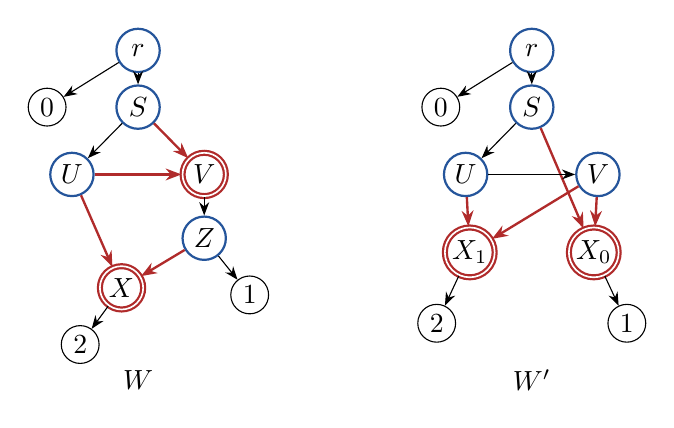
\begin{tikzpicture}[x=1.05cm,y=.9cm,>=Stealth]
  \node[treev] (r) at (0,3) {$r$};
  \node[treev] (S) at (0,2.2) {$S$};
  \node[leaf] (L0) at (-1.1,2.2) {$0$};
  \node[treev] (U) at (-.8,1.25) {$U$};
  \node[reticv] (V) at (.8,1.25) {$V$};
  \node[treev] (Z) at (.8,.35) {$Z$};
  \node[reticv] (X) at (-.2,-.35) {$X$};
  \node[leaf] (L1) at (1.35,-.45) {$1$};
  \node[leaf] (L2) at (-.7,-1.15) {$2$};
  \draw[->] (r)--(S); \draw[->] (r)--(L0);
  \draw[->] (S)--(U); \draw[reticedge] (S)--(V);
  \draw[reticedge] (U)--(V); \draw[reticedge] (U)--(X);
  \draw[->] (V)--(Z); \draw[reticedge] (Z)--(X);
  \draw[->] (Z)--(L1); \draw[->] (X)--(L2);
  \node at (0,-1.65) {$W$};

  \begin{scope}[xshift=5cm]
  \node[treev] (rp) at (0,3) {$r$};
  \node[treev] (Sp) at (0,2.2) {$S$};
  \node[leaf] (L0p) at (-1.1,2.2) {$0$};
  \node[treev] (Up) at (-.8,1.25) {$U$};
  \node[treev] (Vp) at (.8,1.25) {$V$};
  \node[reticv] (X0) at (.75,.15) {$X_0$};
  \node[reticv] (X1) at (-.75,.15) {$X_1$};
  \node[leaf] (L1p) at (1.15,-.85) {$1$};
  \node[leaf] (L2p) at (-1.15,-.85) {$2$};
  \draw[->] (rp)--(Sp); \draw[->] (rp)--(L0p);
  \draw[->] (Sp)--(Up); \draw[reticedge] (Sp)--(X0);
  \draw[->] (Up)--(Vp); \draw[reticedge] (Vp)--(X0);
  \draw[reticedge] (Up)--(X1); \draw[reticedge] (Vp)--(X1);
  \draw[->] (X0)--(L1p); \draw[->] (X1)--(L2p);
  \node at (0,-1.65) {$W'$};
  \end{scope}
\end{tikzpicture}
\end{center}

Put \(\delta=2^{-30}\).  In \(W\), assign \((s,g)=(1/7,1/7)\) to the seven
nonpendant arcs
\[
 rS,SU,SV,UX,VZ,ZX,UV.
\]
At reticulation \(X\), give \(Z\to X\) weight \(15996/16339\) and
\(U\to X\) its complement \(343/16339\).  At \(V\), give \(S\to V\)
weight \(1/8\) and \(U\to V\) weight \(7/8\).  Give the pendant arms at
leaves \(0,1,2\) the strict continuous-time diagonal pairs
\[
 (s,g)=(x_i,x_i),\qquad
 (x_0,x_1,x_2)=
 \left(\frac{86779}{80}\delta,
       \frac{320}{253}\delta,
       \frac{114373}{20240}\delta\right).
\]

In \(W'\), assign \((1/4,1/4)\) to
\[
 rS,SU,SX_0,VX_0,UX_1,VX_1,UV.
\]
At \(X_1\), the edges \(V\to X_1,U\to X_1\) have weights \(1/2,1/2\).
At \(X_0\), the edges \(V\to X_0,S\to X_0\) have weights \(1/6,5/6\).
The pendant diagonal pairs at leaves \(0,1,2\) are
\[
 \left(\frac{16}{3}\delta,\frac{16}{3}\delta\right),\quad
 \left(\frac{32}{9}\delta,\frac{32}{9}\delta\right),\quad
 \left(\frac{96}{5}\delta,\frac{96}{5}\delta\right).
\]
Every pair lies strictly in \(\Dct\).

These parameters are written on the displayed rooted arcs.  When the
artificial root is suppressed, the two incident spectra multiply
coordinatewise; the resulting effective semi-directed edge also remains
strict continuous-time.

Use numeric character codes \(0,C,G,T=0,1,2,3\).  In the explicit coordinate
order
\begin{equation}\label{eq:sharp-order}
 (000,0CC,0GG,C0C,CC0,CGT,CTG,G0G,GCT,GG0),
\end{equation}
direct four-switch expansion gives the same tensor on both networks:
\begin{align*}
 q_{000}&=1,\qquad
 q_h=\delta^2 &&\text{on the six two-nonzero coordinates},\\
 q_h&=\frac45\delta^3 &&\text{on the three all-nonzero coordinates}.
\end{align*}

The graph-derived canonical descendant-signature orders of the seven visible
edge classes are
\[
 \begin{array}{c|ccccccc}
 W&ZX&SV&rS&SU&UV&VZ&UX\\
 W'&VX_1&VX_0&UV&rS&SX_0&SU&UX_1.
 \end{array}
\]
Order each normalized map's full parameter list by the paired \((s,g)\)
coordinates of these seven classes, followed by \(\lambda_0,\lambda_1\).
Thus the named minor columns are
\[
 \begin{aligned}
 W:;&(s_{ZX},g_{ZX},s_{SV},g_{SV},s_{rS},g_{rS},
       s_{SU},g_{SU},s_{UV}),\\
 W':;&(s_{VX_1},g_{VX_1},s_{VX_0},g_{VX_0},s_{UV},g_{UV},
       s_{rS},g_{rS},s_{SX_0}).
 \end{aligned}
\]
All output-row indices below are zero-based in the order
\eqref{eq:sharp-order}; thus row \(0\) is \(q_{000}\).
The derived column crosswalk in the supplement independently reconstructs
these orders from the graph encodings and binds them to the frozen descriptor
hashes.  For \(W\), rows \((1,2,3,5,4,7,6,8,9)\) of
\eqref{eq:sharp-order} and the displayed named columns give determinant
\[
 \frac{10368019213741323}
 {563981315074464023964442388464888915634290688}\ne0.
\]
For \(W'\), rows \((1,2,3,5,4,6,7,8,9)\) and its displayed named columns give
\[
 \frac{1435825}{85002596691653613846528}\ne0.
\]
Both normalized maps therefore have rank nine, the full normalized three-leaf
dimension.  The nonzero pendant factors are an invertible diagonal row
scaling, so both full physical maps are submersions at their common tensor.
Their images share a regular nine-dimensional germ.

To pass from \(n\) leaves to \(n+1\), replace the same labelled leaf on both
networks by the same labelled cherry.  If the two new edge pairs are
\((u_s,u_g)\) and \((v_s,v_g)\), call the new leaves \(a,b\), and choose any
outside leaf \(j\).  On the positive common germ the following Fourier
coordinates are nonzero, and character conservation gives
\[
 R_s=
 \frac{Q_{j=C,a=C,b=0,\,\mathrm{others}=0}}
      {Q_{j=C,a=0,b=C,\,\mathrm{others}=0}}
 =\frac{u_s}{v_s},
 \qquad
 P_s=Q_{a=C,b=C,\,\mathrm{others}=0}=u_sv_s.
\]
Replacing \(C\) by \(G\) gives \(R_g=u_g/v_g\) and \(P_g=u_gv_g\).
Thus the four quantities below are tensor observables, not auxiliary
parameter functions:
\[
 R_s=u_s/v_s,\quad P_s=u_sv_s,\qquad
 R_g=u_g/v_g,\quad P_g=u_gv_g.
\]
Their Jacobian determinant is
\begin{equation}\label{eq:cherry-det}
 \det\frac{\partial(R_s,P_s,R_g,P_g)}
 {\partial(u_s,v_s,u_g,v_g)}
 =\frac{4u_su_g}{v_sv_g}\ne0.
\end{equation}
For example, the actual pairs
\((u_s,u_g)=(2/5,4/9)\) and
\((v_s,v_g)=(3/7,5/11)\) lie in \(\Dct\), and
\eqref{eq:cherry-det} equals \(2464/675\).  The extended tensor factors
through the old tensor and the four new edge coordinates, giving an upper
bound of four new dimensions.  The inverse formulas
\(u_s=\sqrt{R_sP_s}\), \(v_s=\sqrt{P_s/R_s}\), and their \(g\)-sector
analogues recover those four coordinates analytically.  Every old tensor
coordinate is then recovered from a cherry coordinate by dividing by its
corresponding nonzero \(u\)- or \(v\)-factor; the old all-zero coordinate is
one.  Thus these observables together with the old tensor give a local
inverse.  Both extended images contain the image of the same analytic map
from the common old germ times this four-edge chart.  Thus each cherry adds
exactly four dimensions, and iteration gives
\(9+4(n-3)=4n-3\).

A tree-child and a non-tree-child base rooting both lift through every cherry.
Pruning the newest labelled cherry and suppressing its parent returns the base
graph.  Hence weak-not-strong status, level two, binary degree, nonisomorphism,
and failure of triangle equivalence all persist.
\end{proof}

Thus ``strongly'' in \cref{thm:main} cannot be weakened to ``weakly,'' even in
strict continuous time.  The theorem does not say that every weak network is
ambiguous.

\section{Scope, proof status, and reproducibility}\label{sec:status}

The main classification excludes stochastic boundary points, singular edge
eigenvalues, inheritance probabilities zero or one, nonbinary networks,
networks of level greater than two, merely weakly tree-child networks, and
every mixed-sign K2P component outside \(\Dplus\).  It classifies regular
analytic containment germs and generic structural recovery, not full-image
equality, universal numerical-parameter identifiability, noisy-data
estimation, conditioning, or finite-sample model selection.

The finite theorem is supported by a deterministic proof package.  A quick
entry point checks the frozen manifests, exact certificates, cross-layer
censuses, and independent replays.  A full entry point additionally regenerates
the raw four-port and five-port ledgers, rank certificates, direct polynomial
overlay, restoration forest, cycle closure, and one-/two-port probe package
from primitive graph encodings.  Mutations target every load-bearing failure
class listed in the proof of \cref{thm:bounded}.  The supplement records the
exact paths, SHA-256 bindings, environment, and commands.  The theorem relies
on this exact finite computation; ``independent replay'' means a separately
implemented program, not an independent human review.

\section*{Data and code availability}

The exact certificate and replay files are contained in the public repository
\url{https://github.com/AlecKriebel/Math} under
\path{k2p_level2_identifiability_closure}.  The designated versioned annotated
source tag for this submission is \texttt{k2p-same-biorxiv-v1.0.4}; no DOI is
claimed.  Its tag-object and peeled-commit identifiers are recorded in
external release metadata after the final source commit is created.  The
article, supplement, and certificate data are licensed under CC BY 4.0, and
the verifier code is licensed under the MIT License.  The reader
supplement provides a relative-path crosswalk that remains valid in the local
reproducibility tree; the deterministic archive hash is emitted as external
release metadata to avoid a self-referential archive.

\section*{Author contributions}

Alec Kriebel conceived and directed the study, fixed the mathematical scope
and conventions, adjudicated proof and audit results, curated the exact
reproducibility package, and accepts responsibility for the final claims and
submission.

\section*{Funding}

No specific funding supported this work.

\section*{Competing interests}

The author declares no competing interests.

\section*{Use of generative AI}

Generative AI systems assisted with mathematical exploration, code generation,
implementation, drafting, and adversarial review.  Several earlier automated
claims failed audit, including a reciprocal-only bridge chart and incomplete
restoration/probe narratives; those versions are retained only as quarantined
history and are not theorem evidence.  The active claims are supported by
exact graph-derived certificates, direct derivations, separately implemented
replays, and fail-closed mutation tests.  No independent human specialist
review is claimed.  The author accepts responsibility for the mathematical
statement, code, and final submission.

{\small
\bibliographystyle{plain}
\bibliography{references}
}

\end{document}
